%%
%% Copyright 2007, 2008, 2009 Elsevier Ltd
%%
%% This file is part of the 'Elsarticle Bundle'.
%% ---------------------------------------------
%%
%% It may be distributed under the conditions of the LaTeX Project Public
%% License, either version 1.2 of this license or (at your option) any
%% later version.  The latest version of this license is in
%%    http://www.latex-project.org/lppl.txt
%% and version 1.2 or later is part of all distributions of LaTeX
%% version 1999/12/01 or later.
%%
%% The list of all files belonging to the 'Elsarticle Bundle' is
%% given in the file `manifest.txt'.
%%

%% Template article for Elsevier's document class `elsarticle'
%% with numbered style bibliographic references
%% SP 2008/03/01
%%
%%
%%
%% $Id: elsarticle-template-num.tex 4 2009-10-24 08:22:58Z rishi $
%%
%%
\documentclass[final,5p,times,twocolumn]{elsarticle}

%% Use the option review to obtain double line spacing
%% \documentclass[preprint,review,12pt]{elsarticle}

%% Use the options 1p,twocolumn; 3p; 3p,twocolumn; 5p; or 5p,twocolumn
%% for a journal layout:
%% \documentclass[final,1p,times]{elsarticle}
%% \documentclass[final,1p,times,twocolumn]{elsarticle}
%% \documentclass[final,3p,times]{elsarticle}
%% \documentclass[final,3p,times,twocolumn]{elsarticle}
%% \documentclass[final,5p,times]{elsarticle}
%% \documentclass[final,5p,times,twocolumn]{elsarticle}

%% if you use PostScript figures in your article
%% use the graphics package for simple commands
%% \usepackage{graphics}
%% or use the graphicx package for more complicated commands
%% \usepackage{graphicx}
%% or use the epsfig package if you prefer to use the old commands
%% \usepackage{epsfig}

%% The amssymb package provides various useful mathematical symbols
\usepackage{amssymb}
%% The amsthm package provides extended theorem environments
%% \usepackage{amsthm}

%% The lineno packages adds line numbers. Start line numbering with
%% \begin{linenumbers}, end it with \end{linenumbers}. Or switch it on
%% for the whole article with \linenumbers after \end{frontmatter}.
%% \usepackage{lineno}

%% natbib.sty is loaded by default. However, natbib options can be
%% provided with \biboptions{...} command. Following options are
%% valid:

%%   round  -  round parentheses are used (default)
%%   square -  square brackets are used   [option]
%%   curly  -  curly braces are used      {option}
%%   angle  -  angle brackets are used    <option>
%%   semicolon  -  multiple citations separated by semi-colon
%%   colon  - same as semicolon, an earlier confusion
%%   comma  -  separated by comma
%%   numbers-  selects numerical citations
%%   super  -  numerical citations as superscripts
%%   sort   -  sorts multiple citations according to order in ref. list
%%   sort&compress   -  like sort, but also compresses numerical citations
%%   compress - compresses without sorting
%%
%% \biboptions{comma,round}

% \biboptions{}


\journal{Composites}

\begin{document}

\begin{frontmatter}
\title{A Modification of Nonlinear Theory with Equivalent Stiffness for Metal Wire Braid Reinforced Hose}





%\tnoteref{label0}
%\tnotetext[label0]{This is only an example}


%% Author One
\author[addr1]{Ma Pengsheng}


%% Author Two
\author[addr2]{Hu Muyuan}
\ead{charlie.yaha@gmail.com}


%% Author Thre
\author[addr2]{Zheng Bailin\corref{cor1}}
\ead{author.three@mail.com}
\cortext[cor1]{I am corresponding author}



%% Address Ref

\address[addr1]{School Of Material Science And Engineering Tongji University, Shanghai, China}
\address[addr2]{School Of Aerospace Engineering And Applied Mechanics, Tongji University, Shanghai, China}


\begin{abstract}
	We conducted an experiment and put forward several modifications, based on the method proposed in Hachemi’s research of metal wire braid reinforced hose, in order to enhance the constitutive theory, which is discovered not keeping up with the experimental results when it shows far more non-lineal mechanical behavior than the theory predict. We introduced a “modifying matrix”, from composites mechanics, to detach inter-wire contacts from wire elongation, seldom considered before. We also proposed a hypothesis opposite to Hachemi’s: the hose’s braid angle decreased linearly, applied displacement load with constant loading rate, rather than locked at a certain degree. So that we introduce a modification coefficient \textit{k,} accelerating the decrease of braid angle to match the linearity in force-displacement curve. Lateral contact is considered to be the factor of excessively decreased braid angle when the calculated curve perfectly meet the experimental one, with suitable \textit{k}.

\end{abstract}





\begin{keyword}
%% keywords here, in the form: keyword \sep keyword
braid \sep
PTFE \sep 
hose \sep
Elastic-Modulus \sep
Model

%% MSC codes here, in the form: \MSC code \sep code
%% or \MSC[2008] code \sep code (2000 is the default)
\end{keyword}

\end{frontmatter}
%%
%% Start line numbering here if you want
%%
% \linenumbers
%% main text


\section{Introduction}
\label{introduction}

High pressure flexible hoses, reinforced by braided metallic or fabric wires, are utilized in a variety of engineering applications, to transmit fluid in aircrafts, automobiles and typical hydraulic systems. 
These hoses are practically employed in more severe conditions, where high pressure loads, commonly of the order of tens of MPa,  are not static but periodically or randomly fluctuating, and furthermore thermal loading, vibration and large deformation are coupled with the pressure[]. 



The construction of such a hose is illustrated in Fig.\ref{fig:Hose-Structure}. It comprises an inner tube core, mostly PTFE, covered with layers of high tensile steel wires wounding around it, such that the PTFE resists leakage and chemical corrosion while the steel wires layers act as the principle load-carrying elements. These reinforcement layers can be classified into helix-wounds and braids. 






Braided structures can be categorized as diamond ($ 1 \times 1 $ repeat), regular ($ 2 \times 2 $ repeat) and hercules ($ 3 \times 3 $ repeat) based on the weave pattern \cite{Rawal:2015dq}  and the regular braids are most widely produced for high pressure flexible hose on circular braiding machines.
Regular braids  are also known as biaxial braids, consisting of two sets of braider strands, which are aligned in the bias angle to the axis, namely the braid angle, which play a pivot part in defining the performance of the hose under pressure.[1]

\begin{figure}[h]
\centering
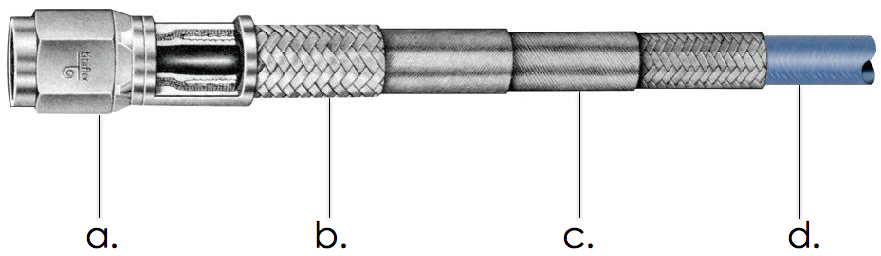
\includegraphics[width=0.7\linewidth]{figures/Hose-Structure}
\caption{Hose Structure}
\label{fig:Hose-Structure}
\end{figure}





The helix-wound layers are wounded in pairs, one layer of each pair being wound left hand and the other right hand in order to achieve a torque balanced construction (i.e. minimal twist on pressurization)[]. There are no intermediate layers of plastic and wires in the same layer are touching in order for maximum packing density.



In conventional braider, spindle carriers rotate along a circular track. Half of the carriers travel in clockwise direction, with the others in the reverse direction, similar to maypole arrangement (see Figure 1).As a result, he two sets of spindles interlace with each other at a bias angle to the tube axis, namely the braid angle, which play a pivot part in defining the performance of the hose under pressure.[1]
The tube in Figure 1 is designed a hybrid structure with both the helix-wound reinforcement and the braid reinforcement, to have sufficient structural safety against extremely high pressure. They may be independently used in middle-high pressure hose. Braided fiber yarns, especially Kevlar [], has been used instead of metallic wires, for its light weight. Effects have been made to model and characterize the mechanical and structural elements of the three reinforcement methods respectively.






\section{Experimental Works}
\label{experiment}



%% The Appendices part is started with the command \appendix;
%% appendix sections are then done as normal sections





\begin{figure}
\centering
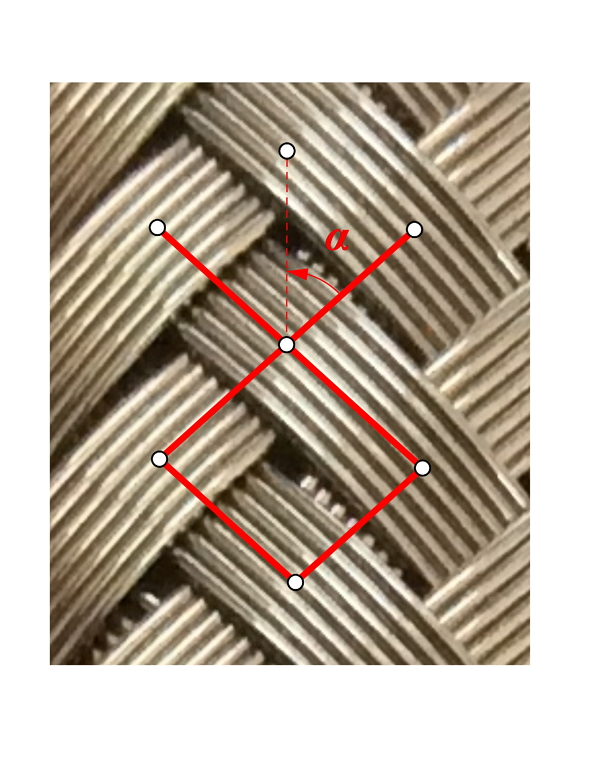
\includegraphics[width=0.7\linewidth]{figures/braid-angle}
\caption{ just have test}
\label{fig:braid-angle}
\end{figure}






%%backmatters
%
%% Reference and appendix

%% Appendix
%\appendix
%\section{Section in Appendix}
%\label{appendix-sec1}

%% References
%%
%% Following citation commands can be used in the body text:
%% Usage of \cite is as follows:
%%   \cite{key}         ==>>  [#]
%%   \cite[chap. 2]{key} ==>> [#, chap. 2]
%%
%% References with bibTeX database:

%\bibliographystyle{elsarticle-num}
 %\bibliographystyle{elsarticle-harv}
\bibliographystyle{elsarticle-num-names}
% \bibliographystyle{model1a-num-names}
% \bibliographystyle{model1b-num-names}
% \bibliographystyle{model1c-num-names}
% \bibliographystyle{model1-num-names}
% \bibliographystyle{model2-names}
% \bibliographystyle{model3a-num-names}
% \bibliographystyle{model3-num-names}
% \bibliographystyle{model4-names}
% \bibliographystyle{model5-names}
% \bibliographystyle{model6-num-names}

\bibliography{main}



\end{document}

%%
%% End of file `elsarticle-template-num.tex'.
